%% current contest NAME

\chapter{One Small Step}
\begin{minipage}[b]{4.25in}
%\begin{quote}
\begin{slshape}
  {\large \textsc{The year is 2067}}. After decades of inefficient,
  bureaucratic attempts to utilize the Solar System's vast mineral
  wealth for the benefit of the burgeoning \textsc{Terran Civilization},
  private corporations and wealthy individuals have taken it upon
  themselves to do what their national governments could not.  
\end{slshape}
\end{minipage}
\hspace*{.25in}
\includegraphics[width=1.5in]{contest/lander.eps}
\begin{slshape}

  Built from off-the-shelf components and proven modular structural
  elements, dozens of \textsc{exploratory robots} have been dispatched
  to the surfaces of Mars and other planetary bodies for a triple
  purpose: to gather \textsc{mineral samples}, searching for valuable
  isotopes like fissile $^{294}_{118}$eka-emanation and fusile $^3_2$He;
  to establish a legal and material \textsc{claim} for the ground of
  their landing zones; and to bring \textsc{glory and profit} to their
  creators.

  You have the opportunity to take part in this epic endeavor! Many
  contestants have gone before you, and along your way you will
  certainly benefit from their wisdom and experience. Depending on your
  landing zone, you may even encounter feeble robotic representatives of
  the old government explorers. As the intellectual offspring of your
  cadre of brilliant scientists and engineers, our new generation of
  robots will run circles around the big-budget dinosaurs they
  deprecate.

\centering\large\textsc{Explore. Acquire. Conquer.}

\end{slshape}

\section{The Table and Scoring}

%% put table description and image HERE
%\begin{figure}[htbp]
%\begin{center}
%
\includegraphics[width=0.8\textwidth]{contest/board.eps}
%\caption{Table}
%\label{table}
%\end{center}
%\end{figure}

%\begin{figure}[htbp]
%\begin{center}
%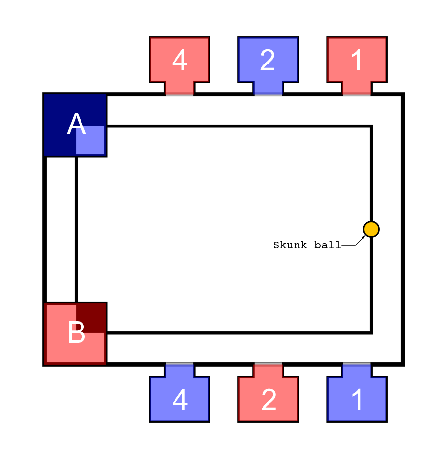
\includegraphics[width=0.8\textwidth]{contest/scoring.eps}
%\caption{Scoring}
%\label{table}
%\end{center}
%\end{figure}

%\begin{figure}[htbp]
%\begin{center}
%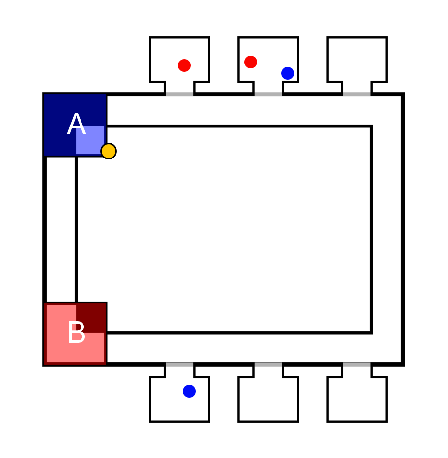
\includegraphics[width=0.8\textwidth]{contest/scoreexample.eps}
%\caption{Scoring example}
%\label{table}
%\end{center}
%\end{figure}

\begin{itemize}

\item The objective of the game is to score as many points as possible for your team. Every robot has a designated goal into which the robot will deliver as many balls as possible.

\item The board contains 14 small balls, and 4 big balls. Small balls are worth 1 point, big balls 4. Note that the board allows for small balls to be rolled into goals, but big balls will need to be lifted over the wall in some manner.

\item In addition to gathering balls, a robot has the opportunity to raise a flag for its team. The flag is raised by interfacing with a rotating gear setup in the flagbox. The robot with a higher flag will have its score doubled!

%[image: scoring]

\item The round ends after 90 seconds of game-play. All points will be evaluated when the board is settled, i.e. when the robots and balls are still. Upon evaluation, the team with the highest score will win.

\end{itemize}

\subsubsection{Tiebreakers}

In the event that two teams have identical scores, we will use the following program to determine the winner:

\begin{enumerate}
\item The team with a higher flag wins. A ``tie'' in flag height favors the player that arrived to the flagbox first.
\item If neither team affects the flag, the player that has scored more large balls wins.
\item If both teams avoided the big balls, a rematch will be awarded if each robot scored \emph{at least} 4 points. Note that in this circumstance, the scores are identical.
\item For a score below 4, a coin toss will determine the winner. 
\end{enumerate}

Note that double wins will not be possible under this scenario.

\subsection{Losing the Round}

\begin{itemize}
\item If the robot failed to favorably affect the game it will lose the round. By ``favorably affect'' we mean either: place a ball in your scoring bin, or raise the flag for your team. The other team does not win by default: there exists the possibilty of double loses.

\item If the robot falls out of the arena (the playing board excluding the scoring zones), it loses the round.
\end{itemize}

Note that there will be scenarios where both competitors lose the match. If neither robot scores any points, nor raises its own flag (regardless of the number of balls scored), then the round results in a double loss.

If you have any questions or comments regarding the rules, please email 6.270-rules@mit.edu. We will get back to you ASAP.

%%put scoring rules HERE^^^

%%% Local Variables: 
%%% mode: latex
%%% TeX-master: "notes"
%%% End: 
